
%% bare_conf.tex
%% V1.3
%% 2007/01/11
%% by Michael Shell
%% See:
%% http://www.michaelshell.org/
%% for current contact information.
%%
%% This is a skeleton file demonstrating the use of IEEEtran.cls
%% (requires IEEEtran.cls version 1.7 or later) with an IEEE conference paper.
%%
%% Support sites:
%% http://www.michaelshell.org/tex/ieeetran/
%% http://www.ctan.org/tex-archive/macros/latex/contrib/IEEEtran/
%% and
%% http://www.ieee.org/

%%*************************************************************************
%% Legal Notice:
%% This code is offered as-is without any warranty either expressed or
%% implied; without even the implied warranty of MERCHANTABILITY or
%% FITNESS FOR A PARTICULAR PURPOSE! 
%% User assumes all risk.
%% In no event shall IEEE or any contributor to this code be liable for
%% any damages or losses, including, but not limited to, incidental,
%% consequential, or any other damages, resulting from the use or misuse
%% of any information contained here.
%%
%% All comments are the opinions of their respective authors and are not
%% necessarily endorsed by the IEEE.
%%
%% This work is distributed under the LaTeX Project Public License (LPPL)
%% ( http://www.latex-project.org/ ) version 1.3, and may be freely used,
%% distributed and modified. A copy of the LPPL, version 1.3, is included
%% in the base LaTeX documentation of all distributions of LaTeX released
%% 2003/12/01 or later.
%% Retain all contribution notices and credits.
%% ** Modified files should be clearly indicated as such, including  **
%% ** renaming them and changing author support contact information. **
%%
%% File list of work: IEEEtran.cls, IEEEtran_HOWTO.pdf, bare_adv.tex,
%%                    bare_conf.tex, bare_jrnl.tex, bare_jrnl_compsoc.tex
%%*************************************************************************

% *** Authors should verify (and, if needed, correct) their LaTeX system  ***
% *** with the testflow diagnostic prior to trusting their LaTeX platform ***
% *** with production work. IEEE's font choices can trigger bugs that do  ***
% *** not appear when using other class files.                            ***
% The testflow support page is at:
% http://www.michaelshell.org/tex/testflow/



% Note that the a4paper option is mainly intended so that authors in
% countries using A4 can easily print to A4 and see how their papers will
% look in print - the typesetting of the document will not typically be
% affected with changes in paper size (but the bottom and side margins will).
% Use the testflow package mentioned above to verify correct handling of
% both paper sizes by the user's LaTeX system.
%
% Also note that the "draftcls" or "draftclsnofoot", not "draft", option
% should be used if it is desired that the figures are to be displayed in
% draft mode.
%
\documentclass[conference]{IEEEtran}
% Add the compsoc option for Computer Society conferences.
%
% If IEEEtran.cls has not been installed into the LaTeX system files,
% manually specify the path to it like:
% \documentclass[conference]{../sty/IEEEtran}





% Some very useful LaTeX packages include:
% (uncomment the ones you want to load)


% *** MISC UTILITY PACKAGES ***
%
%\usepackage{ifpdf}
% Heiko Oberdiek's ifpdf.sty is very useful if you need conditional
% compilation based on whether the output is pdf or dvi.
% usage:
% \ifpdf
%   % pdf code
% \else
%   % dvi code
% \fi
% The latest version of ifpdf.sty can be obtained from:
% http://www.ctan.org/tex-archive/macros/latex/contrib/oberdiek/
% Also, note that IEEEtran.cls V1.7 and later provides a builtin
% \ifCLASSINFOpdf conditional that works the same way.
% When switching from latex to pdflatex and vice-versa, the compiler may
% have to be run twice to clear warning/error messages.






% *** CITATION PACKAGES ***
%
%\usepackage{cite}
% cite.sty was written by Donald Arseneau
% V1.6 and later of IEEEtran pre-defines the format of the cite.sty package
% \cite{} output to follow that of IEEE. Loading the cite package will
% result in citation numbers being automatically sorted and properly
% "compressed/ranged". e.g., [1], [9], [2], [7], [5], [6] without using
% cite.sty will become [1], [2], [5]--[7], [9] using cite.sty. cite.sty's
% \cite will automatically add leading space, if needed. Use cite.sty's
% noadjust option (cite.sty V3.8 and later) if you want to turn this off.
% cite.sty is already installed on most LaTeX systems. Be sure and use
% version 4.0 (2003-05-27) and later if using hyperref.sty. cite.sty does
% not currently provide for hyperlinked citations.
% The latest version can be obtained at:
% http://www.ctan.org/tex-archive/macros/latex/contrib/cite/
% The documentation is contained in the cite.sty file itself.






% *** GRAPHICS RELATED PACKAGES ***
%
\ifCLASSINFOpdf
  \usepackage[pdftex]{graphicx}
  % declare the path(s) where your graphic files are
  % \graphicspath{{../pdf/}{../jpeg/}}
  % and their extensions so you won't have to specify these with
  % every instance of \includegraphics
  % \DeclareGraphicsExtensions{.pdf,.jpeg,.png}
\else
  % or other class option (dvipsone, dvipdf, if not using dvips). graphicx
  % will default to the driver specified in the system graphics.cfg if no
  % driver is specified.
  % \usepackage[dvips]{graphicx}
  % declare the path(s) where your graphic files are
  % \graphicspath{{../eps/}}
  % and their extensions so you won't have to specify these with
  % every instance of \includegraphics
  % \DeclareGraphicsExtensions{.eps}
\fi
% graphicx was written by David Carlisle and Sebastian Rahtz. It is
% required if you want graphics, photos, etc. graphicx.sty is already
% installed on most LaTeX systems. The latest version and documentation can
% be obtained at: 
% http://www.ctan.org/tex-archive/macros/latex/required/graphics/
% Another good source of documentation is "Using Imported Graphics in
% LaTeX2e" by Keith Reckdahl which can be found as epslatex.ps or
% epslatex.pdf at: http://www.ctan.org/tex-archive/info/
%
% latex, and pdflatex in dvi mode, support graphics in encapsulated
% postscript (.eps) format. pdflatex in pdf mode supports graphics
% in .pdf, .jpeg, .png and .mps (metapost) formats. Users should ensure
% that all non-photo figures use a vector format (.eps, .pdf, .mps) and
% not a bitmapped formats (.jpeg, .png). IEEE frowns on bitmapped formats
% which can result in "jaggedy"/blurry rendering of lines and letters as
% well as large increases in file sizes.
%
% You can find documentation about the pdfTeX application at:
% http://www.tug.org/applications/pdftex





% *** MATH PACKAGES ***
%
%\usepackage[cmex10]{amsmath}
% A popular package from the American Mathematical Society that provides
% many useful and powerful commands for dealing with mathematics. If using
% it, be sure to load this package with the cmex10 option to ensure that
% only type 1 fonts will utilized at all point sizes. Without this option,
% it is possible that some math symbols, particularly those within
% footnotes, will be rendered in bitmap form which will result in a
% document that can not be IEEE Xplore compliant!
%
% Also, note that the amsmath package sets \interdisplaylinepenalty to 10000
% thus preventing page breaks from occurring within multiline equations. Use:
%\interdisplaylinepenalty=2500
% after loading amsmath to restore such page breaks as IEEEtran.cls normally
% does. amsmath.sty is already installed on most LaTeX systems. The latest
% version and documentation can be obtained at:
% http://www.ctan.org/tex-archive/macros/latex/required/amslatex/math/





% *** SPECIALIZED LIST PACKAGES ***
%
%\usepackage{algorithmic}
% algorithmic.sty was written by Peter Williams and Rogerio Brito.
% This package provides an algorithmic environment fo describing algorithms.
% You can use the algorithmic environment in-text or within a figure
% environment to provide for a floating algorithm. Do NOT use the algorithm
% floating environment provided by algorithm.sty (by the same authors) or
% algorithm2e.sty (by Christophe Fiorio) as IEEE does not use dedicated
% algorithm float types and packages that provide these will not provide
% correct IEEE style captions. The latest version and documentation of
% algorithmic.sty can be obtained at:
% http://www.ctan.org/tex-archive/macros/latex/contrib/algorithms/
% There is also a support site at:
% http://algorithms.berlios.de/index.html
% Also of interest may be the (relatively newer and more customizable)
% algorithmicx.sty package by Szasz Janos:
% http://www.ctan.org/tex-archive/macros/latex/contrib/algorithmicx/




% *** ALIGNMENT PACKAGES ***
%
%\usepackage{array}
% Frank Mittelbach's and David Carlisle's array.sty patches and improves
% the standard LaTeX2e array and tabular environments to provide better
% appearance and additional user controls. As the default LaTeX2e table
% generation code is lacking to the point of almost being broken with
% respect to the quality of the end results, all users are strongly
% advised to use an enhanced (at the very least that provided by array.sty)
% set of table tools. array.sty is already installed on most systems. The
% latest version and documentation can be obtained at:
% http://www.ctan.org/tex-archive/macros/latex/required/tools/


%\usepackage{mdwmath}
%\usepackage{mdwtab}
% Also highly recommended is Mark Wooding's extremely powerful MDW tools,
% especially mdwmath.sty and mdwtab.sty which are used to format equations
% and tables, respectively. The MDWtools set is already installed on most
% LaTeX systems. The lastest version and documentation is available at:
% http://www.ctan.org/tex-archive/macros/latex/contrib/mdwtools/


% IEEEtran contains the IEEEeqnarray family of commands that can be used to
% generate multiline equations as well as matrices, tables, etc., of high
% quality.


%\usepackage{eqparbox}
% Also of notable interest is Scott Pakin's eqparbox package for creating
% (automatically sized) equal width boxes - aka "natural width parboxes".
% Available at:
% http://www.ctan.org/tex-archive/macros/latex/contrib/eqparbox/





% *** SUBFIGURE PACKAGES ***
%\usepackage[tight,footnotesize]{subfigure}
% subfigure.sty was written by Steven Douglas Cochran. This package makes it
% easy to put subfigures in your figures. e.g., "Figure 1a and 1b". For IEEE
% work, it is a good idea to load it with the tight package option to reduce
% the amount of white space around the subfigures. subfigure.sty is already
% installed on most LaTeX systems. The latest version and documentation can
% be obtained at:
% http://www.ctan.org/tex-archive/obsolete/macros/latex/contrib/subfigure/
% subfigure.sty has been superceeded by subfig.sty.



%\usepackage[caption=false]{caption}
%\usepackage[font=footnotesize]{subfig}
% subfig.sty, also written by Steven Douglas Cochran, is the modern
% replacement for subfigure.sty. However, subfig.sty requires and
% automatically loads Axel Sommerfeldt's caption.sty which will override
% IEEEtran.cls handling of captions and this will result in nonIEEE style
% figure/table captions. To prevent this problem, be sure and preload
% caption.sty with its "caption=false" package option. This is will preserve
% IEEEtran.cls handing of captions. Version 1.3 (2005/06/28) and later 
% (recommended due to many improvements over 1.2) of subfig.sty supports
% the caption=false option directly:
%\usepackage[caption=false,font=footnotesize]{subfig}
%
% The latest version and documentation can be obtained at:
% http://www.ctan.org/tex-archive/macros/latex/contrib/subfig/
% The latest version and documentation of caption.sty can be obtained at:
% http://www.ctan.org/tex-archive/macros/latex/contrib/caption/




% *** FLOAT PACKAGES ***
%
%\usepackage{fixltx2e}
% fixltx2e, the successor to the earlier fix2col.sty, was written by
% Frank Mittelbach and David Carlisle. This package corrects a few problems
% in the LaTeX2e kernel, the most notable of which is that in current
% LaTeX2e releases, the ordering of single and double column floats is not
% guaranteed to be preserved. Thus, an unpatched LaTeX2e can allow a
% single column figure to be placed prior to an earlier double column
% figure. The latest version and documentation can be found at:
% http://www.ctan.org/tex-archive/macros/latex/base/



%\usepackage{stfloats}
% stfloats.sty was written by Sigitas Tolusis. This package gives LaTeX2e
% the ability to do double column floats at the bottom of the page as well
% as the top. (e.g., "\begin{figure*}[!b]" is not normally possible in
% LaTeX2e). It also provides a command:
%\fnbelowfloat
% to enable the placement of footnotes below bottom floats (the standard
% LaTeX2e kernel puts them above bottom floats). This is an invasive package
% which rewrites many portions of the LaTeX2e float routines. It may not work
% with other packages that modify the LaTeX2e float routines. The latest
% version and documentation can be obtained at:
% http://www.ctan.org/tex-archive/macros/latex/contrib/sttools/
% Documentation is contained in the stfloats.sty comments as well as in the
% presfull.pdf file. Do not use the stfloats baselinefloat ability as IEEE
% does not allow \baselineskip to stretch. Authors submitting work to the
% IEEE should note that IEEE rarely uses double column equations and
% that authors should try to avoid such use. Do not be tempted to use the
% cuted.sty or midfloat.sty packages (also by Sigitas Tolusis) as IEEE does
% not format its papers in such ways.





% *** PDF, URL AND HYPERLINK PACKAGES ***
%
%\usepackage{url}
% url.sty was written by Donald Arseneau. It provides better support for
% handling and breaking URLs. url.sty is already installed on most LaTeX
% systems. The latest version can be obtained at:
% http://www.ctan.org/tex-archive/macros/latex/contrib/misc/
% Read the url.sty source comments for usage information. Basically,
% \url{my_url_here}.





% *** Do not adjust lengths that control margins, column widths, etc. ***
% *** Do not use packages that alter fonts (such as pslatex).         ***
% There should be no need to do such things with IEEEtran.cls V1.6 and later.
% (Unless specifically asked to do so by the journal or conference you plan
% to submit to, of course. )


% correct bad hyphenation here
\hyphenation{op-tical net-works semi-conduc-tor}


\begin{document}
%
% paper title
% can use linebreaks \\ within to get better formatting as desired
\title{Adult-Size Humanoid Robot Throwing the First Pitch at a Major League Baseball Game \\ A Road Map}


% author names and affiliations
% use a multiple column layout for up to three different
% affiliations
\author{\IEEEauthorblockN{Daniel M. Lofaro}
\IEEEauthorblockA{Electrical and Computer Engineering\\
Drexel University\\
Philadelphia, PA, USA\\
Email: dan@danLofaro.com}
\and
\IEEEauthorblockN{Paul Oh}
\IEEEauthorblockA{Mechanical Engineering\\
Drexel University\\
Philadelphia, PA, USA\\
Email: paul@coe.drexel.edu}
%\and
%\IEEEauthorblockN{Jun-Ho Oh}
%\IEEEauthorblockA{Mechanical Engineering\\
%Korea Advanced Institute of\\Science and Technology\\
%Daejeon, South Korea\\
%Email: jhoh@kaist.ac.kr}
}



% conference papers do not typically use \thanks and this command
% is locked out in conference mode. If really needed, such as for
% the acknowledgment of grants, issue a \IEEEoverridecommandlockouts
% after \documentclass

% for over three affiliations, or if they all won't fit within the width
% of the page, use this alternative format:
% 
%\author{\IEEEauthorblockN{Michael Shell\IEEEauthorrefmark{1},
%Homer Simpson\IEEEauthorrefmark{2},
%James Kirk\IEEEauthorrefmark{3}, 
%Montgomery Scott\IEEEauthorrefmark{3} and
%Eldon Tyrell\IEEEauthorrefmark{4}}
%\IEEEauthorblockA{\IEEEauthorrefmark{1}School of Electrical and Computer Engineering\\
%Georgia Institute of Technology,
%Atlanta, Georgia 30332--0250\\ Email: see http://www.michaelshell.org/contact.html}
%\IEEEauthorblockA{\IEEEauthorrefmark{2}Twentieth Century Fox, Springfield, USA\\
%Email: homer@thesimpsons.com}
%\IEEEauthorblockA{\IEEEauthorrefmark{3}Starfleet Academy, San Francisco, California 96678-2391\\
%Telephone: (800) 555--1212, Fax: (888) 555--1212}
%\IEEEauthorblockA{\IEEEauthorrefmark{4}Tyrell Inc., 123 Replicant Street, Los Angeles, California 90210--4321}}




% use for special paper notices
%\IEEEspecialpapernotice{(Invited Paper)}




% make the title area
\maketitle


\begin{abstract}
%\boldmath
Three different approaches of having an adult-size humanoid robot throw the first pitch at a Major League Baseball game are tested and implemented.  The approaches include kinematic mapping using a motion capture system to capture a human's throwing motion then mapping that to the humanoid robot adult-size humanoid robot Hubo.  The second approach is a fully automated approach that uses the sparse reachable map to provide viable full body throwing trajectories to give the end effector the desired velocity.  The third approach borrows from the animation industry.  Key frames of the desired trajectory is constructed by hand.  The time between each key frame is defined by the user.  A forth order interpolation method is used to smoothly move from key frame to key frame while limiting the jerk.  Each method is analyzed and tested in simulation and on physical hardware.  Based on the latter tests one method was chosen to throw a successful first pitch.
\end{abstract}
% IEEEtran.cls defaults to using nonbold math in the Abstract.
% This preserves the distinction between vectors and scalars. However,
% if the conference you are submitting to favors bold math in the abstract,
% then you can use LaTeX's standard command \boldmath at the very start
% of the abstract to achieve this. Many IEEE journals/conferences frown on
% math in the abstract anyway.

% no keywords




% For peer review papers, you can put extra information on the cover
% page as needed:
% \ifCLASSOPTIONpeerreview
% \begin{center} \bfseries EDICS Category: 3-BBND \end{center}
% \fi
%
% For peerreview papers, this IEEEtran command inserts a page break and
% creates the second title. It will be ignored for other modes.
\IEEEpeerreviewmaketitle

\section{Introduction}
% no \IEEEPARstart
In early February 2012 the director of the Philadelphia Science Festival asked the Drexel Autonomous Systems Lab (DASL)\footnote{Drexel Autonomous Systems Lab: http://dasl.mem.drexel.edu}\label{foot:dasl} if they could have their adult-size humanoid robot Jaemi Hubo throw the ceremonial first pitch at the second annual \textit{Science Night at the Ballpark}.  On April 28th, 2012 Hubo successfully threw the first pitch at the Philadelphia Phillies Vs. Chicago Cubs game, see Fig.~\ref{fig:hubo-throw}.  

\begin{figure}[t]
  \centering
\includegraphics[width=1.0\columnwidth]{./pix/hubo-pitch.png}
  \caption{Hubo successfully throwing the first pitch at the second annual Philadelphia Science Festival event Science Night at the Ball Park on April 28th, 2012.  The game was between the Philadelphia Phillies and the Chicago Cubs and played at the Major League Baseball stadium Citizens Bank Park.  The Phillies won 5-2}
  \label{fig:hubo-throw}
\end{figure}

Hubo was the first adult-size humanoid robot to throw the first pitch at a Major League baseball game.  The PhillieBot\footnote{PhillieBot Video: http://youtu.be/ShId-vZ-ZEY} made by the GRASP Lab at the University of Pennsylvania was the robot that threw the first pitch at the first annual Philadelphia Science Festival \textit{Science Night at the Ballpark} in 2011.  

This document describes, analyses and tests three different approaches to having an adult-size humanoid robot throw the first pitch.  
Section~\ref{sec:background} gives a brief introduction to work already done in the field as well as states the requirements for the pitch.
Section~\ref{sec:methodology} describes the three different methods tested where:
Section~\ref{sec:sec:mocap} describes the kinematic mapping approach that uses a motion capture system to capture a human's throwing motion then mapping that to an adult-size humanoid robot.  
Section~\ref{sec:sec:srm} describes a fully automated approach that uses the sparse reachable map (SRM) to provide viable full body throwing trajectories to provide the end effector with the desired velocity\cite{dlofaro-srm}.
Section~\ref{sec:sec:keyframe} describes the final method explored which is based on key-frame trajectories.
Section~\ref{sec:comparison} Compares the tests and analyses of each of the methods.
Section~\ref{sec:finalDesign} describes in detain the remainder of the hurtals needed to be overcome to throw a successful pitch using the method chosen in Section~\ref{sec:comparison}.
Finally Section~\ref{sec:conclusion} gives final thoughts and possible improvements for future years.


%% remember robust and to say that you learned from upenns mistakes etc.
\section{Background and Objectives}\label{sec:background}
The location the thrown object (for this document it will be a ball) lands is determined by the velocity (magnitude and direction) of the end-effector and the location of the ball at the release point.  There are many examples of throwing/pitching machines made by commercial companies such as Louisville Slugger $^{TM}$, Jugs$^{TM}$, and Atec$^{TM}$ to name a few.  These devices typically contain one to two fly wheels that the ball travels through in order to be launched or a spring loaded arm that is compressed and released.  Robots designed for throwing come in many shapes and sizes depending on the objective.  2-DOF mechanisms are able to throw in $R^3$ space with the correct kinematic structure.  Such a mechanism can choose its release point or its end-effector velocity but not both.  Mechanisms containing 3 or more DOF with the correct kinematic structure are able to throw in $R^3$ and choose both the release point and the end-effector velocity simultaneously.

% need to modify
Low degree of freedom throwing machines/robots are common.  Typical throwing robots have between one and three degrees of freedom (DOF)~\cite{509405, Lynch97dynamicnonprehensile, 5152525, 509335, springerlink:10.1007/s10015-006-0401-0}.  All of these mechanisms are limited to throwing in a plane.   Sentoo et al.~\cite{4651142} achieved an end-effector velocity of 6.0 m/s and can throw in $R^3$ space using it's Barret Technology Inc 4-DOF arm with a $360^o$ rotation base yaw actuator.  These low degree of freedom throwing robots are either physically attached/planted to the mechanical ground or have a base that is significantly more massive then the arm. 

Haddadin et al.\cite{6094757} used their 7-DOF arm and a 6-DOF force torque sensor with standard feedback methods to dribble a basket ball.  In addition Zhikun et al.~\cite{6094892} used reinforcement learning to teach their 7-DOF planted robot arm to play ping-pong.  Likewise Schaal et al.~\cite{schaal01/BIRG} taught their high degree of freedom (30-DOF) humanoid robot to hit a tennis ball using on-line special statistical learning methods.  Visual feedback was used in the basketball throwing robot by Hu et al.~\cite{5649335} achieving accuracy an of 99\%.  All of the latter robots were fixed to the ground to guarantee stability.

Kim et al. \cite{5686315,JooH2011438} takes the research to the next level with finding optimal overhand and sidearm throwing motions for a high degree of freedom humanoid computer model.  The model consists of 55-DOF and is not fixed to mechanical ground or a massive base.  Motor torques are then calculated to create both sidearm and overhand throws that continuously satisfies the zero-moment-point stability criteria~\cite{4309277}.  

The highly articulated 40-DOF adult size humanoid robot Jaemi Hubo KHR-4 (Fig.~\ref{fig:huboOneFoot}) is the platform focused on in this work.  Jaemi Hubo is a high-gain, position-controlled biped humanoid robot weighing 37kg and standing 130cm tall.  It is designed and made by Dr. Jun-Ho Oh director of the Hubo Lab at the Korean Advanced Institute of Science and Technology (KAIST).  Jaemi has been located at the Drexel Autonomous Systems Lab (DASL) at Drexel University since Fall of 2008.  DASL has extensive experience with the Jaemi Hubo KHR-4 platform in key areas needed to complete this work.  Balancing was explored when developing a real-time zero moment point (ZMP) preview control system for stable walking~\cite{5686276}.  A full-scale safe testing environment designed for experiments with Jaemi Hubo was created using DASL's Systems Integrated Sensor Test Rig (SISTR)~\cite{5686325}.  Additionally all algorithms are able to be tested on miniature and virtual versions of Jaemi Hubo prior to testing on the full-size humanoid robot through the creation of a surrogate testing platform for humanoid robots~\cite{5379582}.
\section{Methodology}\label{sec:methodology}
\subsection{Balance and Stability}\label{sec:sec:balance}
Each of the methods used have to be stable through the motion in order for the system to be stable (i.e. not to fall down).  
The well known zero-moment-point (ZMP) criteria is what each method must adhere to in order to stay statically stable\cite{Vukobratovic19721}.  
To handle perturbation an active balance controller was added.  
The active balance controller is applied on top of the pre-defined trajectories.  
Hubo is modeled as a single inverted pendulum with the center of mass (COM) located at length $L$ from the ankle.  
The compliance of the robot is composed of a spring $K$ and a damper $C$, see Fig.~\ref{fig:invPen}.  
An IMU located at the COM gives the measured orientation.

\begin{figure}[t]
  \centering
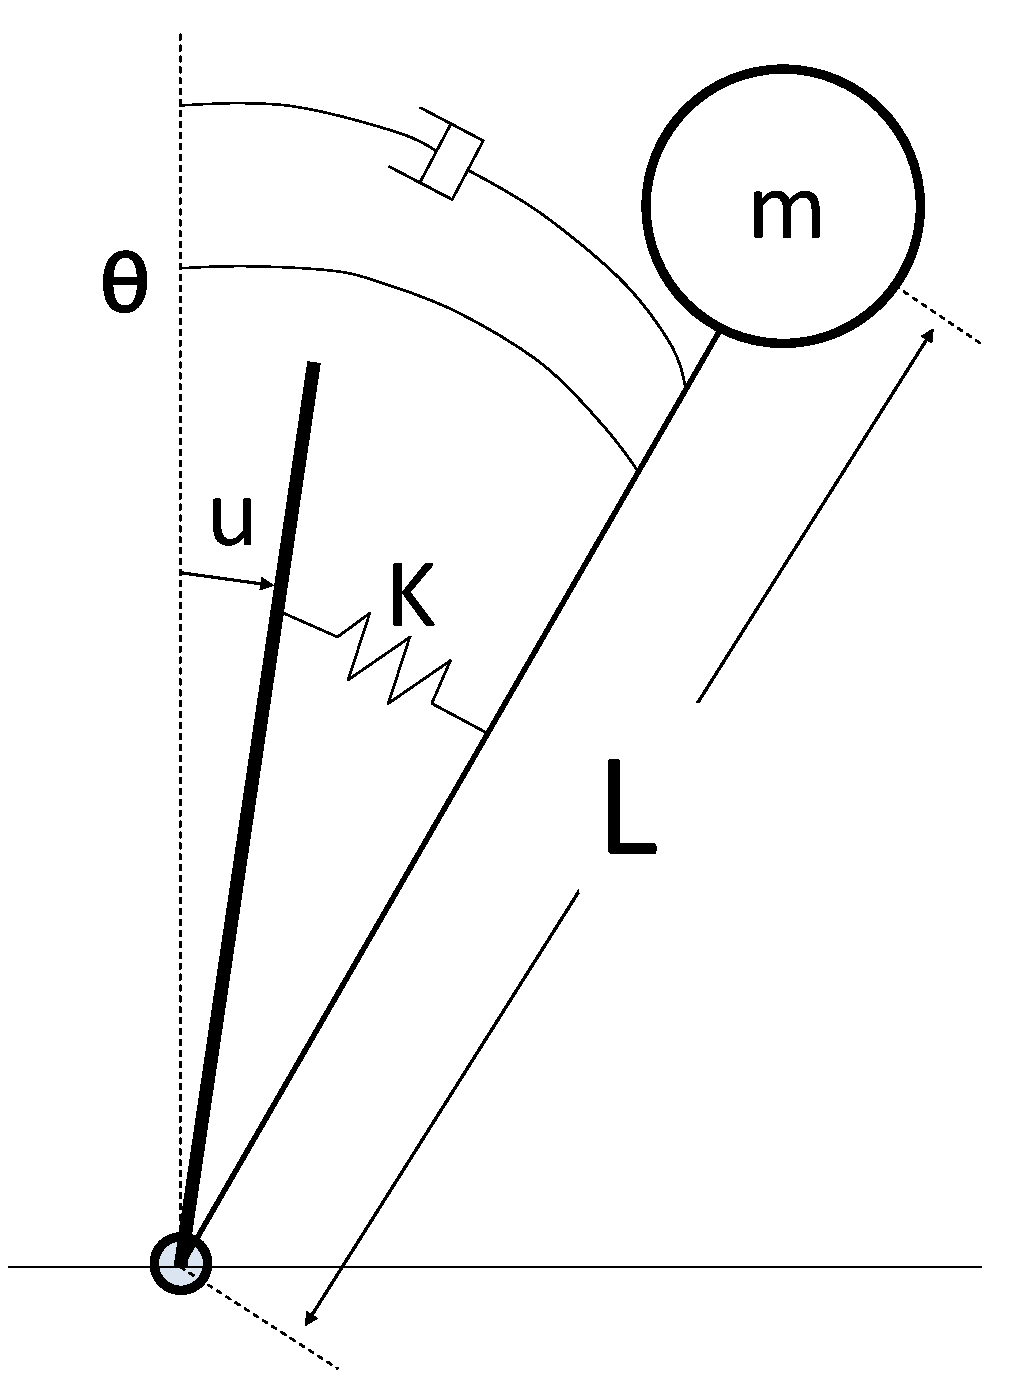
\includegraphics[width=1.0\columnwidth]{./pix/invPen3.pdf}
  \caption{Hubo modeled as a single inverted pendulum with COM located a distance $L$ from }
  \label{fig:invPen}
\end{figure}

The dynamic equation of the simplified model is assumed to be the same in both the sagittal and coronal plane.

\begin{equation}
mL^2\ddot{\theta}+C\dot{\theta}-K\theta = Ku
\end{equation}

This can be linearized and made into the transfer function:

\begin{equation}
%G(s) = \frac{\Theta(s)}{U(s)} = \frac{K}{ mL^2s^2 + Cs + (K - mgL)}
G(s) = \frac{\Theta(s)}{U(s)} = \frac{\frac{K}{mL^2}}{s^2+\frac{C}{mL^2}s + \frac{K-mgL}{mL^2}}
\end{equation}

Prior work on the model and controller for the Hubo by Cho et. al. calculated $K=753\frac{Nm}{rad}$ and $C=18\frac{Nm}{sec}$ using the free vibration response method\cite{5379574}.


\begin{figure}[ht]
  \centering
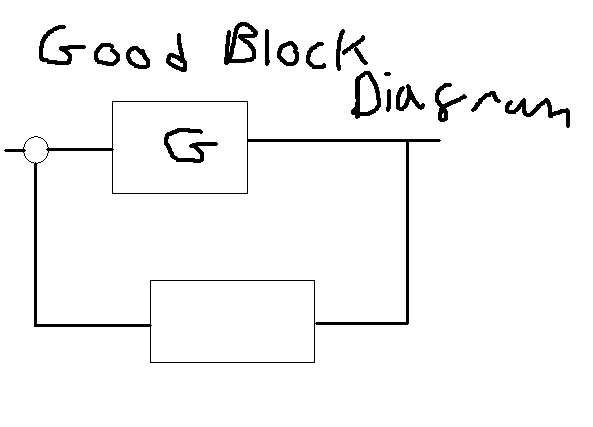
\includegraphics[width=1.0\columnwidth]{./pix/blockDiagram.png}
  \caption{Hubo successfully throwing the first pitch at the second annual Philadelphia Science Festival event Science Night at the Ball Park on April 28th, 2012.  The game was between the Philadelphia Phillies and the Chicago Cubs and played at the Major League Baseball stadium Citizens Bank Park.  The Phillies won 5-2}
  \label{fig:ctrlBlockDiagram}
\end{figure}

The control law is as follows
%ffFor the ankle roll (in the coronal plane) it is always assumed that the desired orientation of the COM is zero degrees.  Thus the roll of the IMU is taken as the error.

\begin{equation}
\theta_{n}^x = \theta_{t}^x + \left(K_p^x+sK_d^x\right)\left(\sum \theta_{t}^x - \theta_{c}^x\right)
%\theta_{n}^x = \theta_{t}^x + (K_p^x+sK_d^x)(\sum \theta_{t}^x - \theta_{c}^x)
%\theta_{new} = \theta_{traj} + (K_p+sK_d)(\sum \theta_{leg} - \theta_{IMU})
\end{equation}

Where $\theta_t$ is the desired trajectory of the lower body (pitch or roll) and $x$ denotes pitch or roll.  $\theta_{c}$ is the orientation of the center of mass in the global frame.  $\theta_n$ is the resulting trajectory.  $K_p$ and $K_d$ are the proportional and derivative gains.  The resulting control allows for a stable stance even with perturbations from upper body motions.

\subsection{Human to Humanoid Robot Kinematic Mapping}\label{sec:sec:mocap}

Motion capture systems are increasingly developed and used as important tool insports training and roboticsto generate human-like motion. 
There exist enormous robotics researches that reply on motion capture data. 
From the sport training perspective, the motion capture system is utilized for example to monitor the movement and reconstruct the movement on a synthetic model. 
[mirabella] The focus is on kinematics analysis to improve and transmitting skill in a sport [1][2][3][4]. 
The key research area in robotics is more of retargeting and execution on the robot than kinematics analysis of the motion data.  
Various approaches for generation of human-like motion for humanoid robots were proposed [qiang][pollard][stefan]. 
Most of the approaches use 3D marker positions as the starting point of data collection.
Stefan et al attempt to use an intermediate model(Master Motor Map) to decouple motion capture data from further post-processing tasks. 
However this added in another conversion to the overall process which causes data lose. 
On the other hand, the motion capture system we adopted auto-generates a lower DoF skeleton from the 3D marker clouds. 
This makes the data collected closer to what we want, and can be seen as a non-physical intermediate model which converts high DoF human motion to lower DoF skeleton motion generated by motion capture system. 
%As many of the mentioned researches above are done in case of relatively slow motion, the high-speed throwing motion which requires high dynamic stability becomes a main concern. The ground contact constraints proposed in [qiang] points out the key issue in the dynamic stability.

Our method for mapping human motion to humanoid motion incorporates the following stages: 1) Human motion capture. 2) Kinematics mapping. 3) Dynamic mapping. 
A motion capture system used in the experiment consists of eighteen cameras with VGA resolution running at 100fps. 
It is able to record the full body motion using thirty-eight reflective markers placed on the actor's body. 
The system creates a 3D cloud of marker points at the rate of 100hz in sub-millimeter precision. 
These 3D points are labeled and mapped to a skeleton of twenty two bones with specifications of the actor's body. 
The skeleton is a human body representation in the motion capture system. 
In this way, the position and the rotation of the bones are obtained in each frame.
The rotation of each bone in the local frame is given in quaternions.% with respect to the end tip of the previous bone.
Kinematics mapping has to resolve three key issues: 
\begin{itemize}
	\item The difference in the total degree of freedom (DOF). 
	\item	The difference in the kinematics descriptions. 
	\item	Kinematic constraints for the robot.
\end{itemize}

The difference in number of bones (linkages) as well as the DOF for each joint caused the difference in the total DOF. 
In reality, all anatomic joints for a human have six DOF []. 
Humans also have soft tissues and vertebra that create more DOF []. 
The skeleton generated does not have soft tissues, it replaced the vertebra with three bones and Hubo has only one DOF(yaw) in between the neck and the hip. 
The key to a successful kinematics mapping will then be to deliver the main information as close as possible and estimate the rest. 
Hence for the underhand throwing motion, the yaw angle of Hubo's waist is the combination of the two joints' yaw angles of the human skeleton.  %% what two joints
The difference in kinematics descriptions lies in the joint configuration. 
(The gross movement of the limb segments interconnected by joints where for the Jaemi HUBO the relative joint rotation is described by adopting the Eulerian angle system, for the human skeleton, Quaternions are used.) 
For Hubo, the finite rotation of joint in the two bone segments is sequence dependent while for human skeleton, the associated three-dimensional finite rotation is sequence independent.
Unlike the generated skeleton in the motion capture system where each joint has multiple DOF, Hubo is constructed with single DOF joints. This makes the joint orientations follow a specific sequence during conversion. For example, from the shoulder to the upper arm, the sequence for shoulder joints is pitch, roll and yaw.  If we move roll prior to pitch, it won't affect the pitch axis but will change the yaw axis.

\begin{figure}[t]
  \centering
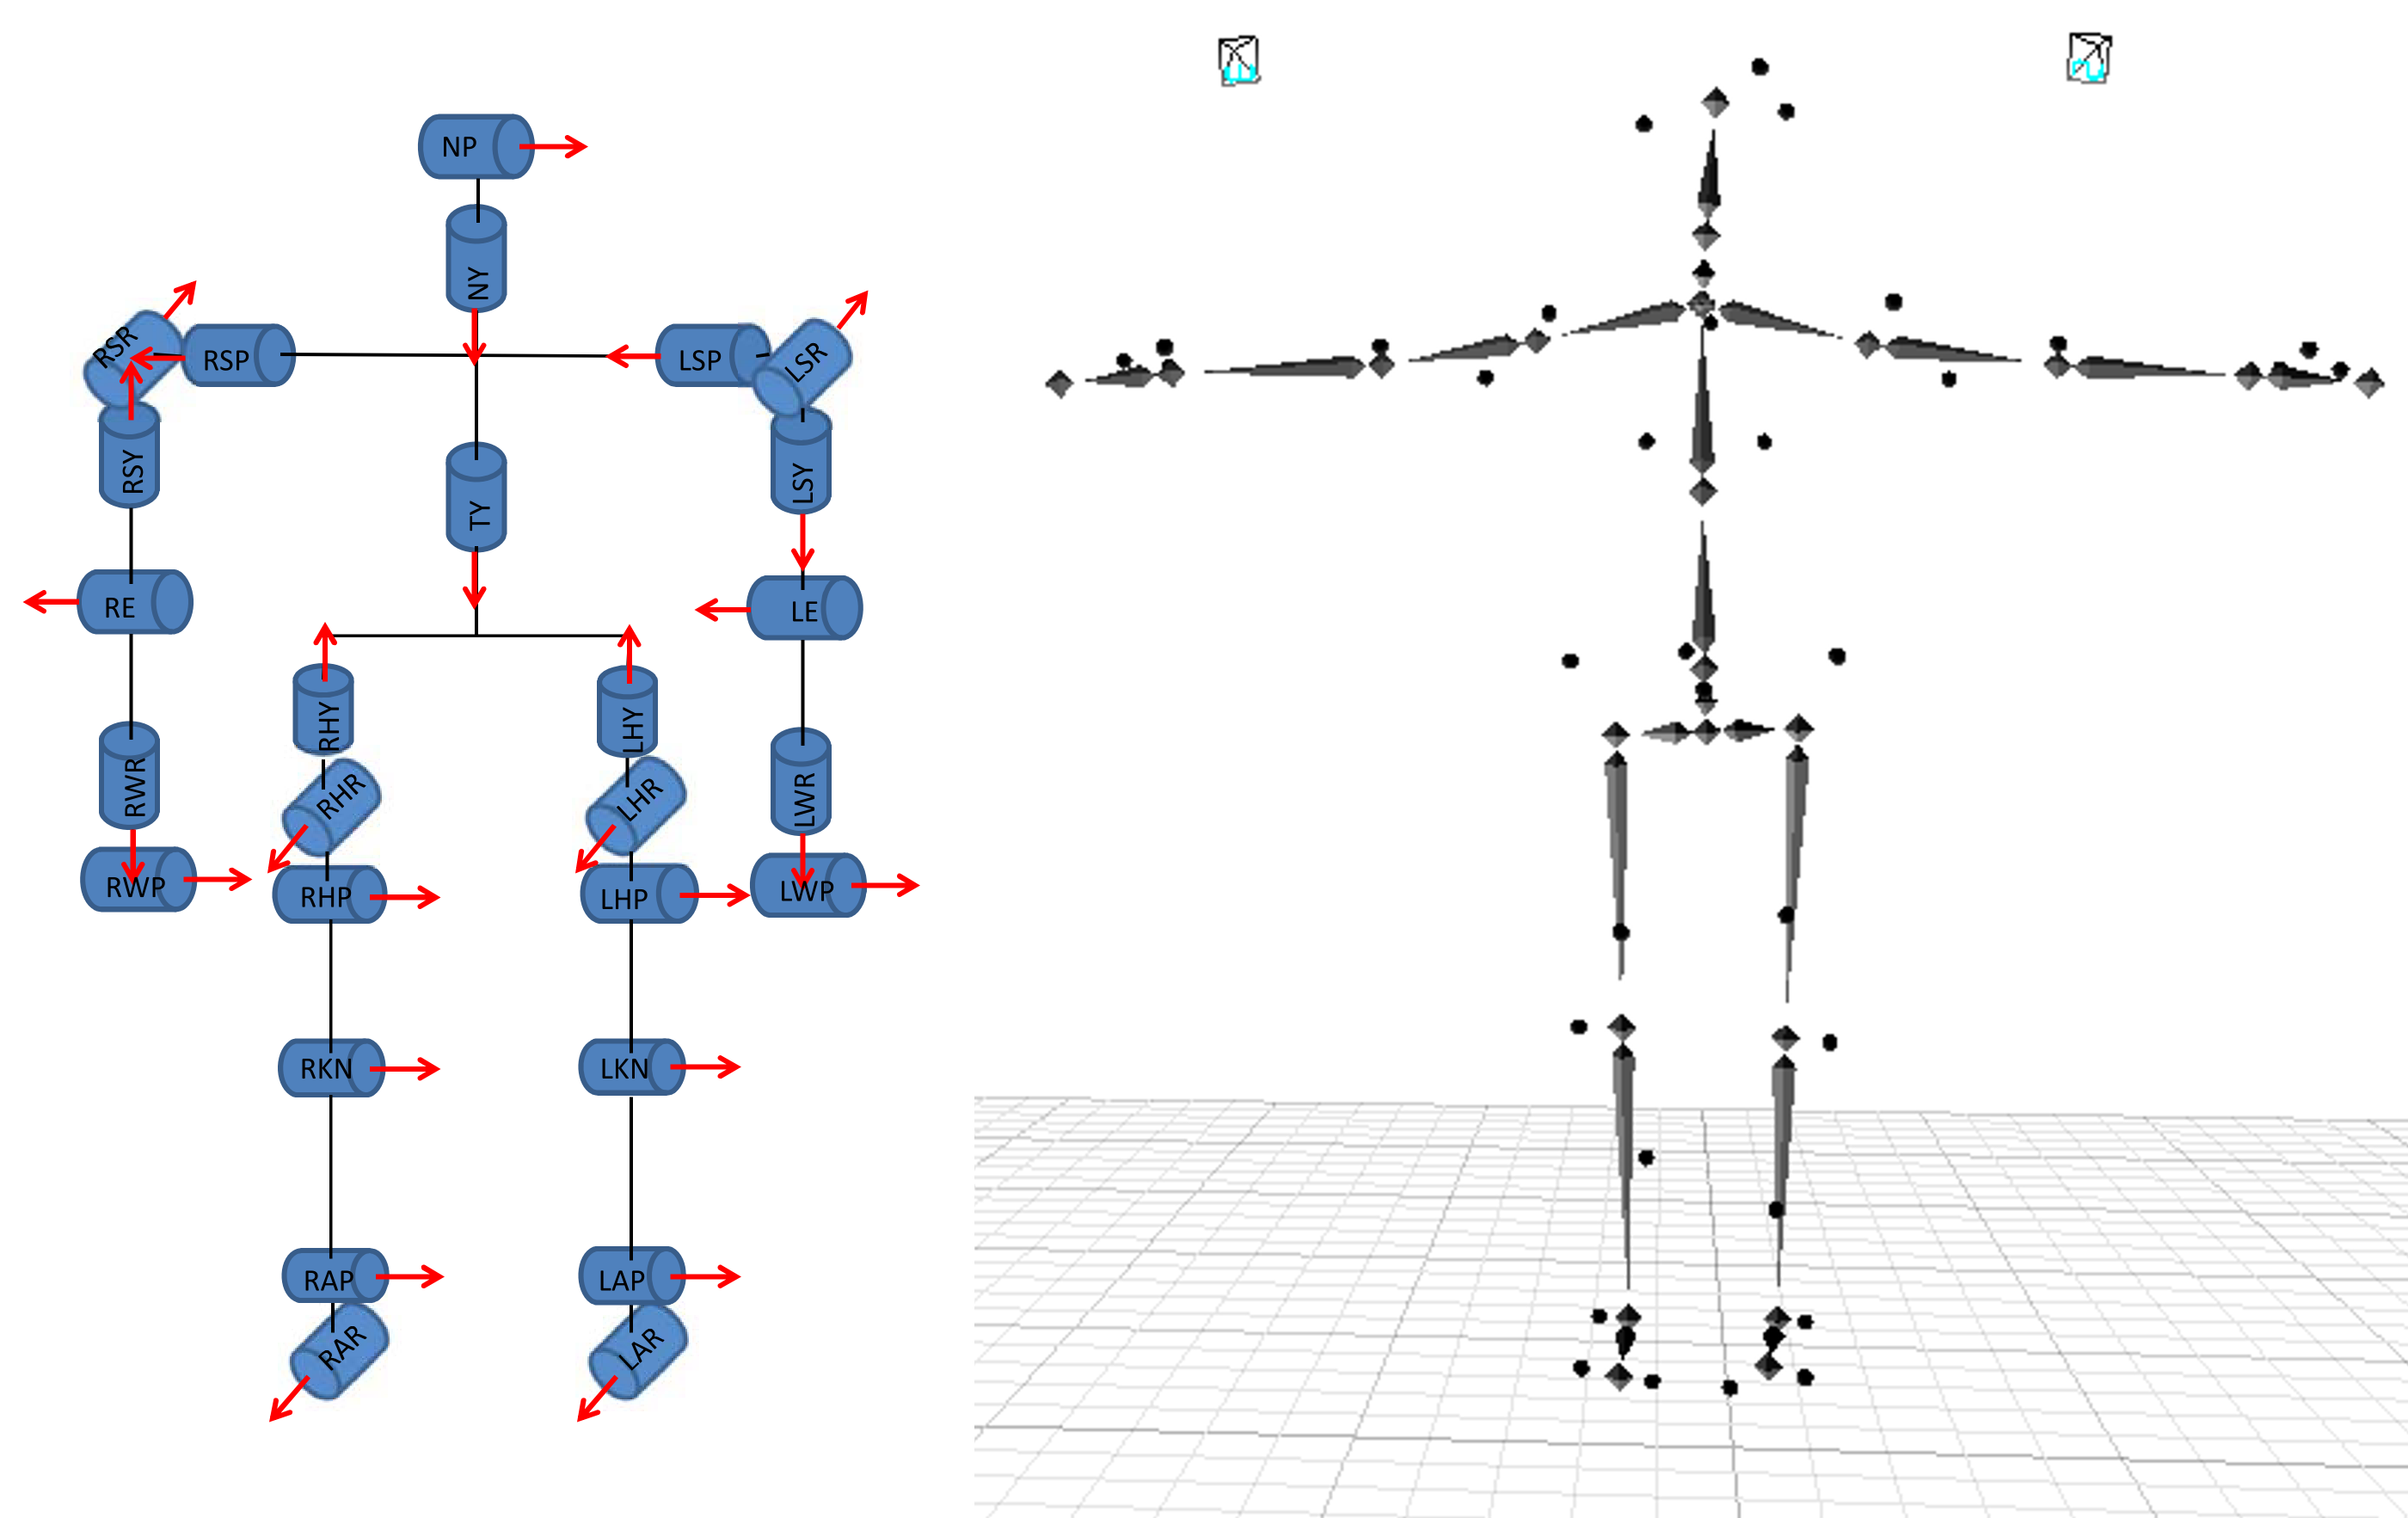
\includegraphics[width=1.0\columnwidth]{./pix/mocapJoints.png}
  \caption{Left: Jaemi Hubo joint order and orientation using right hand rule.  Right: Skeleton generated from motion capture system.  Each joint has three degrees of freedom described via Quaternions in the local frame.}
  \label{fig:mocap-joints}
\end{figure}

Kinematics constraints for the robot include joint angle range and limb contact. 
The kinematics mapping starts from the conversion from quaternions used in motion capture generated skeleton to Euler angles used in Hubo. 
We mainly solve two problems during conversion.  1) Unlike quaternion representation, Euler angles are determined by 24 conventions.  The joint orientation matters for the robot.  Therefore to generate the mapping for a given set of Euler angles, we map rotating axis ri, rj, rk to reference axis i, j, k in the appropriate order.  2) Singularities are generated in conversion from quaternions to Eulerian angle system. When the pitch angle approaches +90 degrees, singularities may occur. We use two methods to avoid singularities. First, use an approximated function for the singularity zone. Second, choose a favorable sequence for joints that have less than three orientations for the robot.
Convention zxy: 
double test = qw*qx + qy*qz;
if (test > 0.499) // singularity at north pole
		yaw = (float) 2.0f * atan2(qy,qw);
		pitch = 3.14159265f/2.0f;
		roll = 0;

if (test < -0.499) // singularity at south pole
		yaw = (float) -2.0f * atan2(qy,qw);
		pitch = - 3.14159265f/2.0f;
		roll = 0;
        

    double sqx = qx*qx;
    double sqy = qy*qy;
    double sqz = qz*qz;
yaw = (float) atan2((double)2.0*qw*qz-2.0*qx*qy , (double)1 - 2.0*sqz - 2.0*sqx);
pitch = (float)asin(2.0*test);
roll = (float) atan2((double)2.0*qw*qy-2.0*qx*qz , (double)1.0 - 2.0*sqy - 2.0*sqx);



\subsection{Throwing Using Sparse Reachable Map}\label{sec:sec:srm}

A Sparse Reachable Map (SRM) is used to create a collision free trajectories while having the end-effector reach a desired velocity as discribed in Lofaro et. al.\cite{dlofaro-srm}.
The SRM has been shown to be a viable method for trajectory generation for high degree of freedom, high-gain position controlled robots.  This remains true when operating without full knowledge of the reachable area as long as a good collision model of the robot is available. 
The end-effector velocity (magnitude and direction) is specified as well as a duration of this velocity. 
The SRM is created by making a sparse map of the reachable end-effector positions in free space and the corresponding poses in joint space by using random sampling in joint space and forward kinematics. 
The desired trajectory in free space is placed within the sparse map with the first point of the trajectory being a known pose from the original sparse map. 

\begin{equation}
L_d(0) \in SRM
\end{equation}

$L_d(0)$ is known both in joint space and in free space.
The Jacobian Transpose Controller method of inverse kinematics as described by Wolovich et al.\cite{4048118} is then used to find the subsequent joint space values for the free space points in the trajectory. 

\begin{equation}
q_1 = q_0 + \dot{q}_0 = q_0 + kJ^Te|_{x_0}^{x_1}
\end{equation}

Where $q_0$ and $x_0$ is the current pose and corresponding end-effector position respectively.  $q_1$ is the next pose for the next desired end-effector position $x_1$.
Each desired end-effector position $x$ must be within a euclidean distance $d$ (user defined) from any point in the SRM.

\begin{equation}
min \left(|x - SRM| \right) < d
\end{equation}

If one of the points in $x$ fails this criteria a new random point is chosen for $L_d(0)$ and the process is repeated.

Each pose in the trajectory is checked against the collision model to guarantee no self-collisions.  The collision model is based on the OpenRAVE model of the Hubo platform called OpenHUBO, see Fig~\ref{fig:vHubo}.

\begin{figure}[ht]
  \centering
%\includegraphics[width=0.5\columnwidth]{./pictures/hubo1s.png}\includegraphics[width=0.5\columnwidth]{./pictures/hubo2s.png}
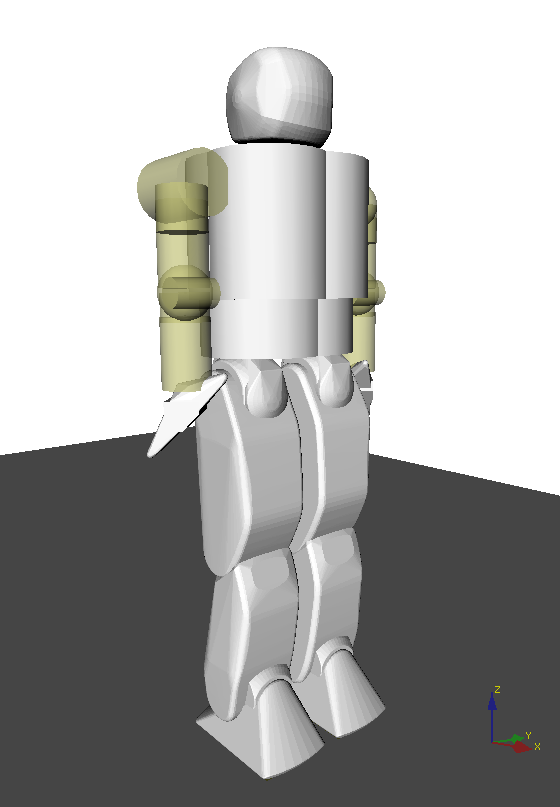
\includegraphics[width=0.5\columnwidth]{./pix/hCol.png}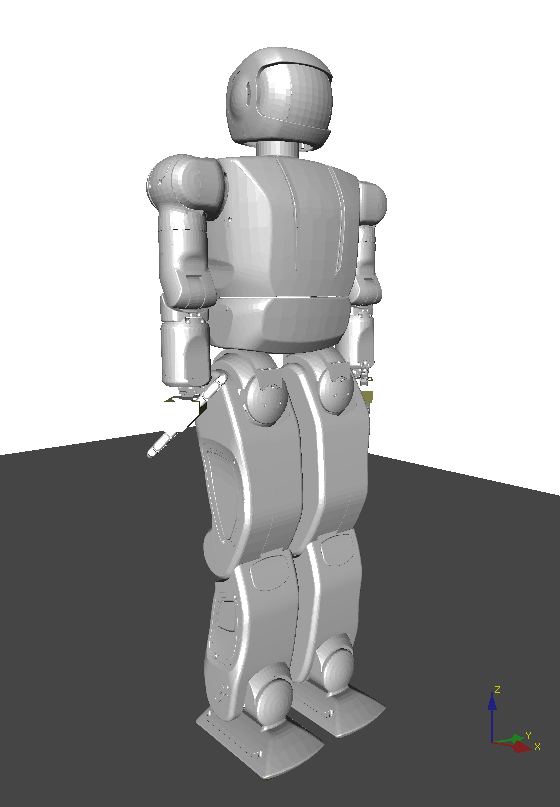
\includegraphics[width=0.5\columnwidth]{./pix/hBody.png}
  \caption{OpenHUBO - OpenRAVE model of Hubo KHR-4.  Left: Collision Geometry.  Right: Model with protective shells\cite{dlofaro-srm}.  }
  \label{fig:vHubo}
\end{figure}

The commanded trajectory produces the desired velocity of 4.9 m/s at 60$^o$.  This was then tested on the OpenHUBO and on the Jaemi Hubo platform, Fig~\ref{fig:fThrow} and Fig~\ref{fig:3dThrowReal} respectively.



\begin{figure}[ht]
  \centering
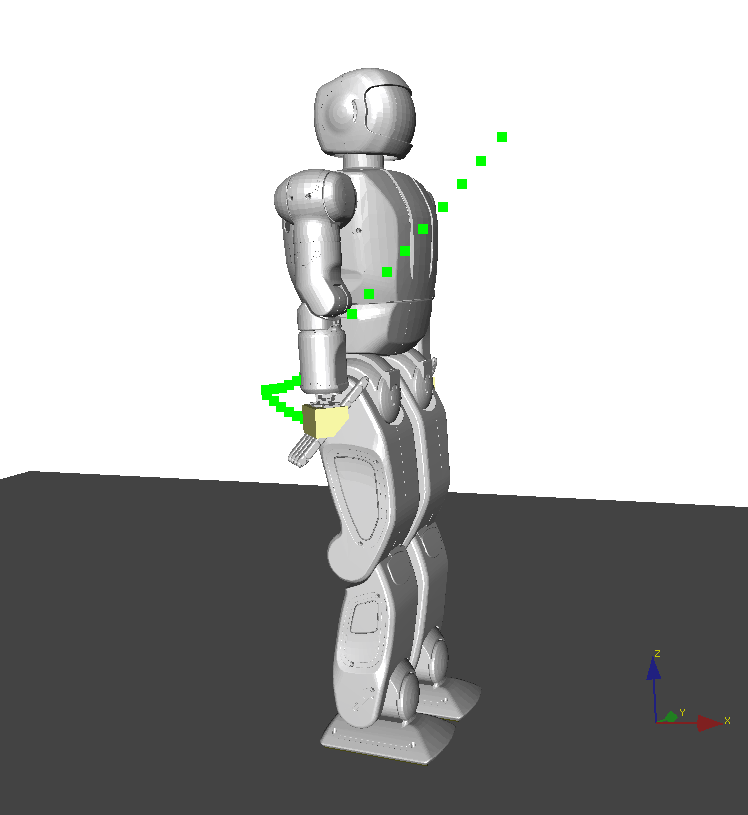
\includegraphics[width=0.25\columnwidth]{./pix/ddFinal/vHside1.png}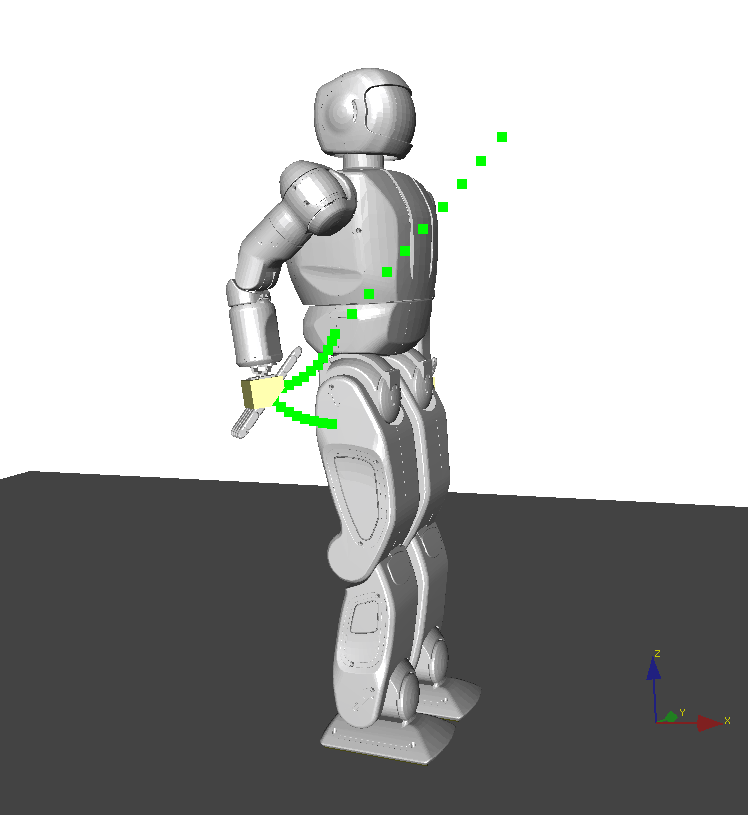
\includegraphics[width=0.25\columnwidth]{./pix/ddFinal/vHside3.png}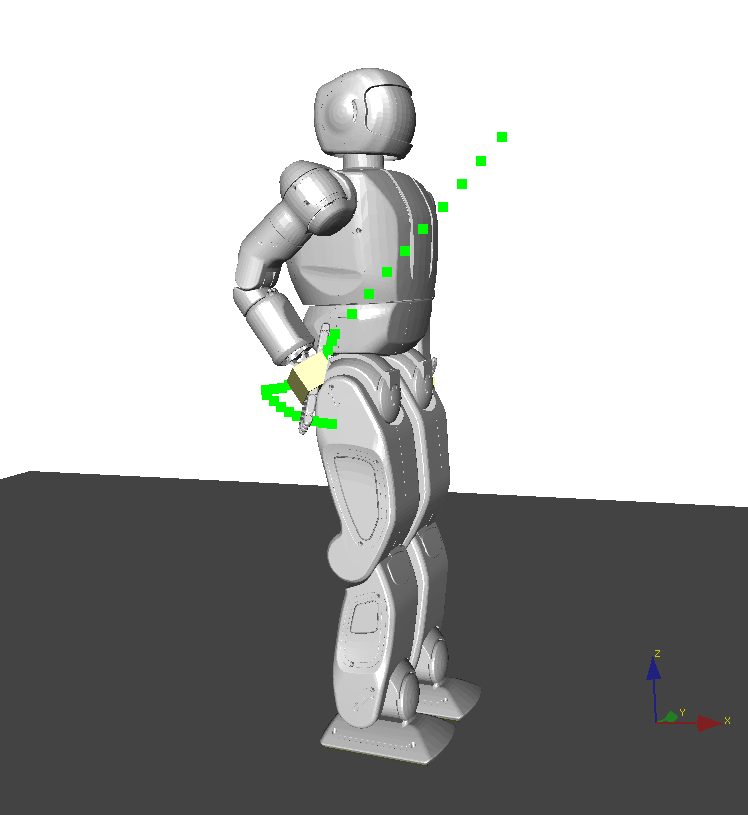
\includegraphics[width=0.25\columnwidth]{./pix/ddFinal/vHside4.png}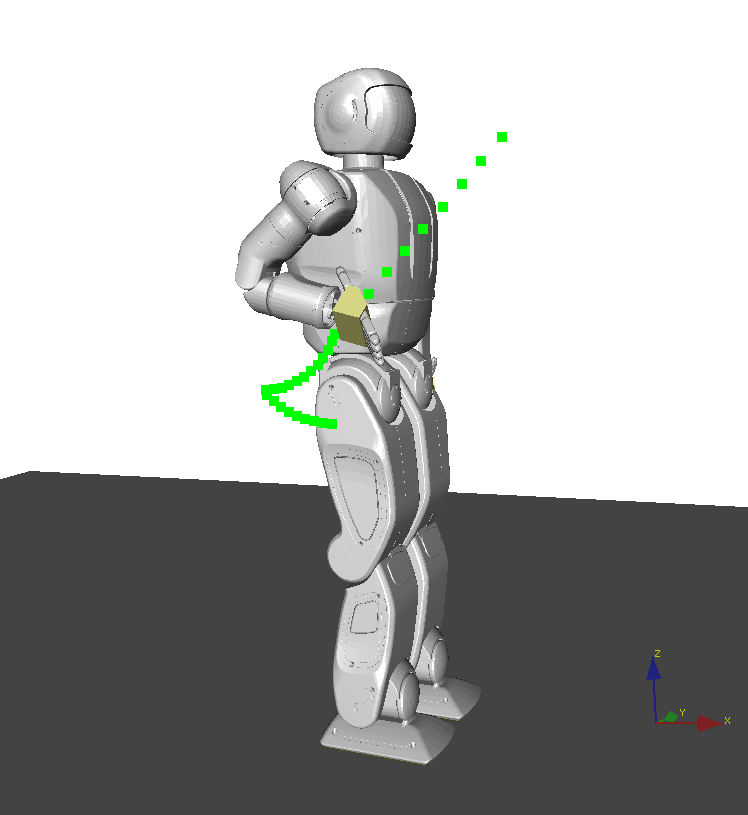
\includegraphics[width=0.25\columnwidth]{./pix/ddFinal/vHside5.png}
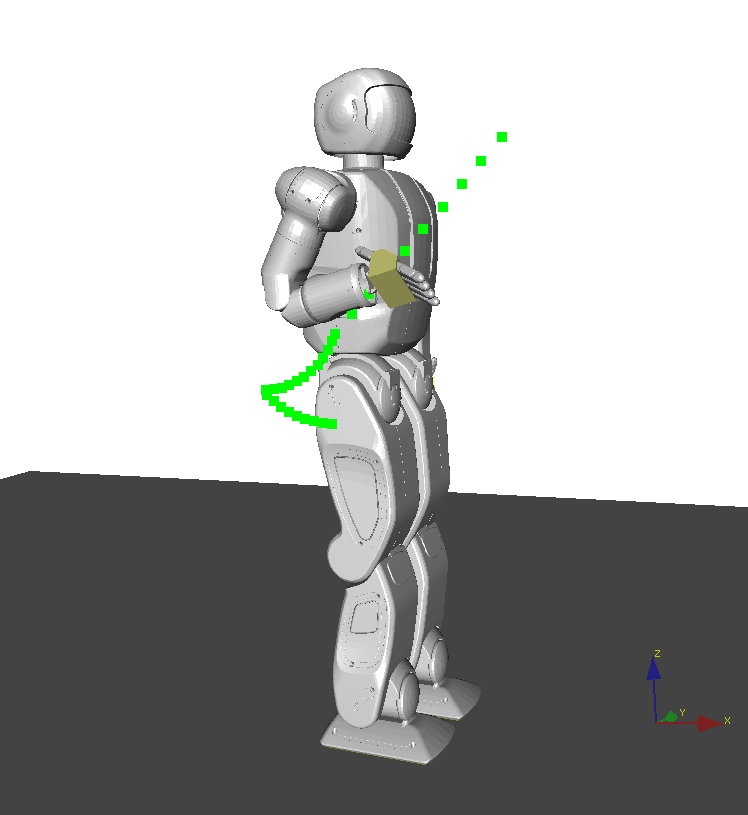
\includegraphics[width=0.25\columnwidth]{./pix/ddFinal/vHside6.png}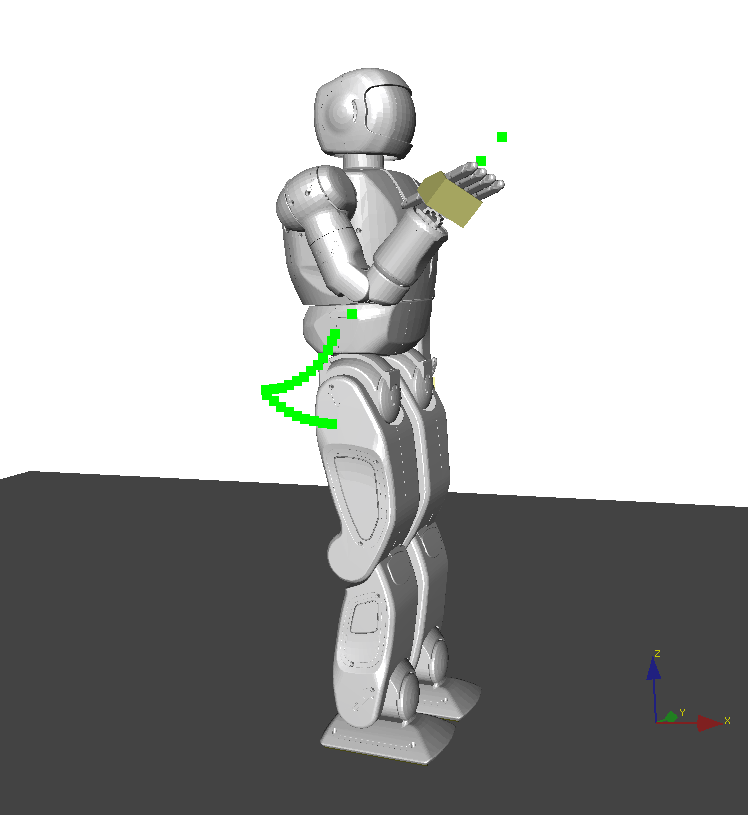
\includegraphics[width=0.25\columnwidth]{./pix/ddFinal/vHside7.png}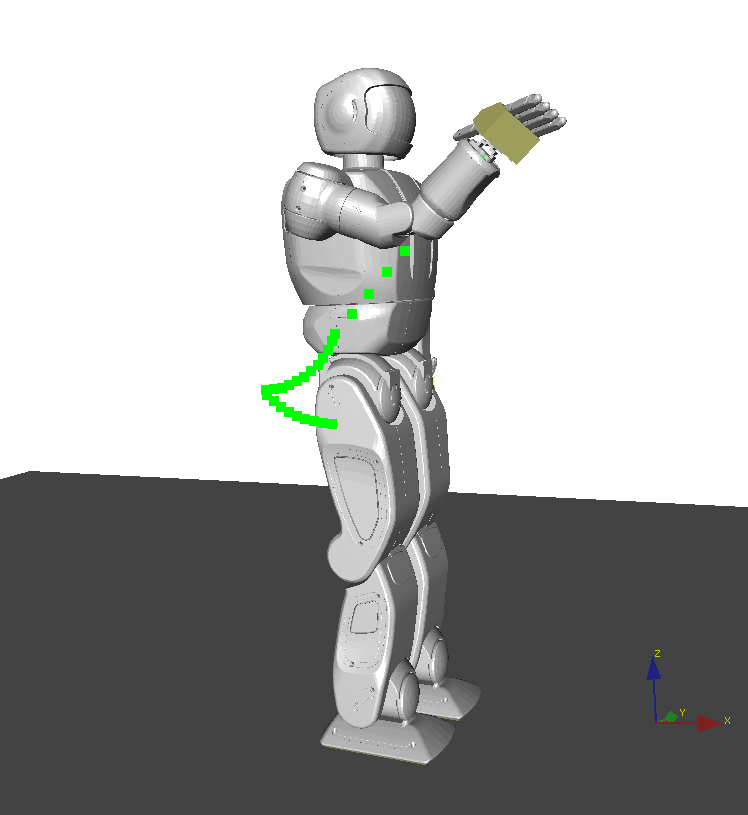
\includegraphics[width=0.25\columnwidth]{./pix/ddFinal/vHside9.png}
  \caption{OpenHUBO running the throwing trajectory immediately after the setup phase is completed.  $x_0$ is top left.  Frames are read left to right and have a $\Delta t$ of 0.15s\cite{dlofaro-srm}}
  \label{fig:fThrow}
\end{figure}

\begin{figure}[ht]
  \centering
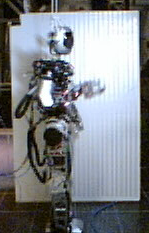
\includegraphics[width=0.25\columnwidth]{./pix/slowMotion/1.png}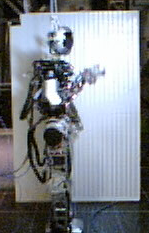
\includegraphics[width=0.25\columnwidth]{./pix/slowMotion/2.png}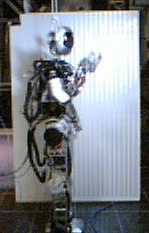
\includegraphics[width=0.25\columnwidth]{./pix/slowMotion/3.png}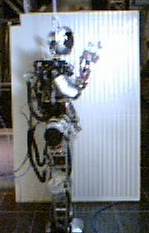
\includegraphics[width=0.25\columnwidth]{./pix/slowMotion/4.png}
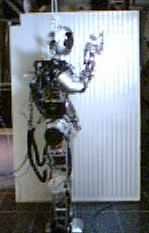
\includegraphics[width=0.25\columnwidth]{./pix/slowMotion/5.png}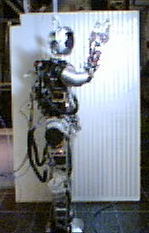
\includegraphics[width=0.25\columnwidth]{./pix/slowMotion/6.png}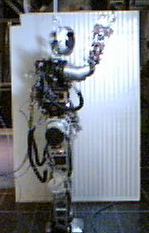
\includegraphics[width=0.25\columnwidth]{./pix/slowMotion/7.png}
  \caption{Jaemi Hubo running the throwing trajectory immediately after the setup phase is completed.  $x_0$ is top left.  Frames are read left to right and have a $\Delta t$ of 0.15 sec\cite{dlofaro-srm}}
  \label{fig:3dThrowReal}
\end{figure}

To ensure balance throughout the motion the balance controller as described in Section~\ref{sec:sec:balance} was applied and the static ZMP criteria was checked for the entire trajectory.
This method worked as desired.  
In approximately 10\% of the tests one or more joints would over torque and shutdown.  
This is due to the system not taking the robots power limitations into account. 


\subsection{Key-Frame Motion}\label{sec:sec:keyframe}

Key-frame motion profiles for humanoid robots borrows from the animation industries' long used techniques.  
When making an animation the master artist/cartoonist will create the character in the most important (or key) poses.  
The apprentice will draw all of the frames between the key poses.  
We borrowed this technique when we: posed the robot in the desired pose, record the values in joint space, and make a smooth motion between poses.  
In place of the apprentice, forth order interpolation methods were used to make smooth trajectories between poses.  
Forth order interpolation was used in order to limit the jerk on each of the joints.  
The resulting trajectory is a smooth well defined motion as seen in Fig.~\ref{fig:keyframe-throw}.

\begin{figure}[t]
  \centering
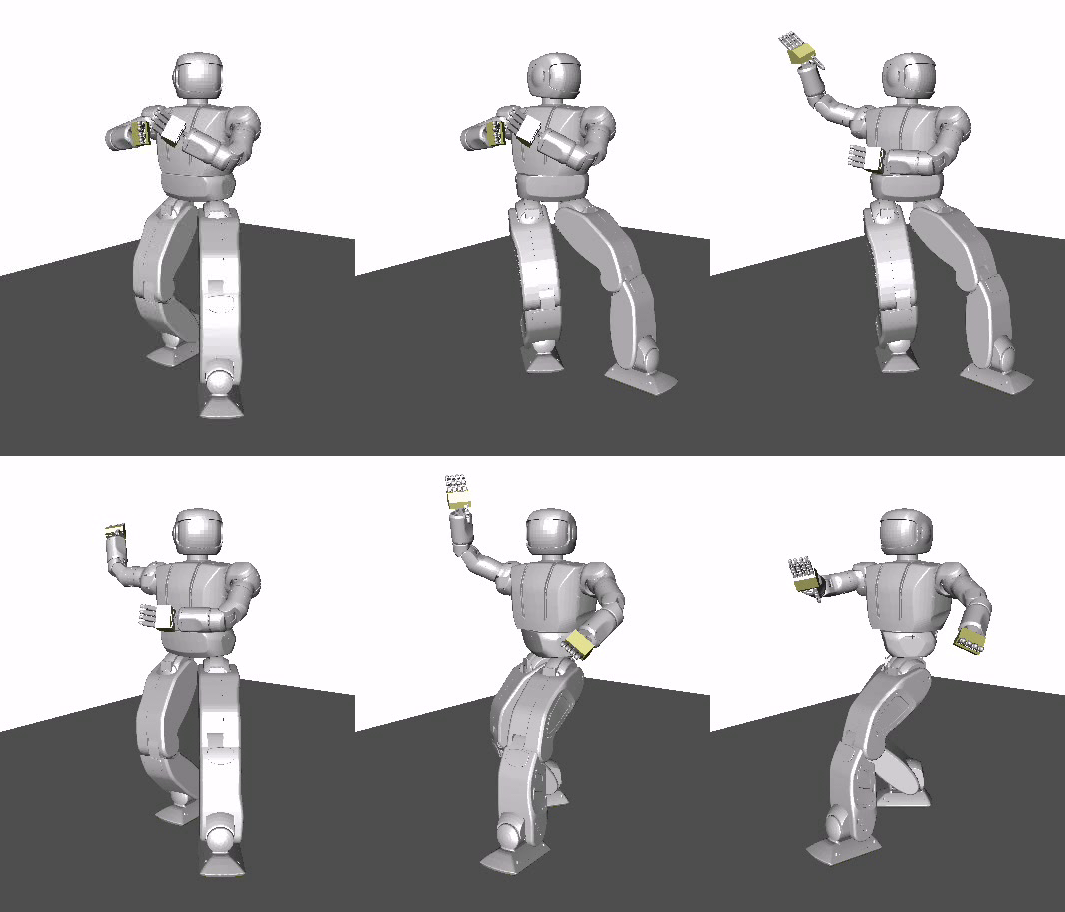
\includegraphics[width=1.0\columnwidth]{./pix/keyframe/keyframe.png}
  \caption{OpenHUBO using key-frame based method for throwing trajectory creation.  Frames are read from top left to bottom right.}
  \label{fig:keyframe-throw}
\end{figure}

To ensure stability throughout the motion the balance controller as described in Section~\ref{sec:sec:balance} was applied and the static ZMP criteria was checked for the entire trajectory.
The resulting end effector velocity was $4.8\frac{m}{s}$ at the release point.  
Fig.~\ref{fig:keyframe-graph} shows the plot of the magnitude of the end effector's velocity.  
It should be noted that at the instance of release the velocity vector is at an elevation of $40^o$ from the ground.

\begin{figure}[t]
  \centering
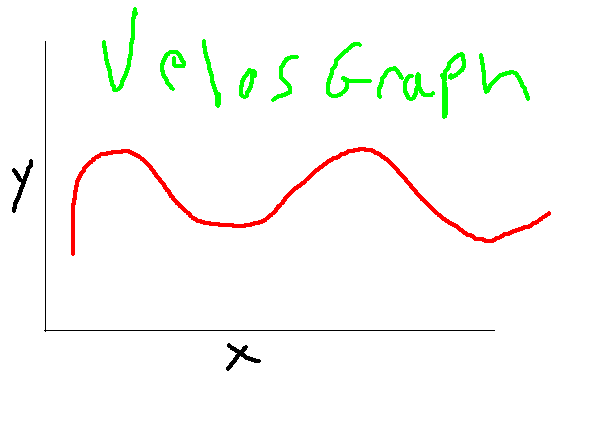
\includegraphics[width=1.0\columnwidth]{./pix/keyframeVelosGraph.png}
  \caption{key-frame throw velocity graph}
  \label{fig:keyframe-graph}
\end{figure}



\section{Results}\label{sec:finalDesign}




% An example of a floating figure using the graphicx package.
% Note that \label must occur AFTER (or within) \caption.
% For figures, \caption should occur after the \includegraphics.
% Note that IEEEtran v1.7 and later has special internal code that
% is designed to preserve the operation of \label within \caption
% even when the captionsoff option is in effect. However, because
% of issues like this, it may be the safest practice to put all your
% \label just after \caption rather than within \caption{}.
%
% Reminder: the "draftcls" or "draftclsnofoot", not "draft", class
% option should be used if it is desired that the figures are to be
% displayed while in draft mode.
%
%\begin{figure}[!t]
%\centering
%\includegraphics[width=2.5in]{myfigure}
% where an .eps filename suffix will be assumed under latex, 
% and a .pdf suffix will be assumed for pdflatex; or what has been declared
% via \DeclareGraphicsExtensions.
%\caption{Simulation Results}
%\label{fig_sim}
%\end{figure}

% Note that IEEE typically puts floats only at the top, even when this
% results in a large percentage of a column being occupied by floats.


% An example of a double column floating figure using two subfigures.
% (The subfig.sty package must be loaded for this to work.)
% The subfigure \label commands are set within each subfloat command, the
% \label for the overall figure must come after \caption.
% \hfil must be used as a separator to get equal spacing.
% The subfigure.sty package works much the same way, except \subfigure is
% used instead of \subfloat.
%
%\begin{figure*}[!t]
%\centerline{\subfloat[Case I]\includegraphics[width=2.5in]{subfigcase1}%
%\label{fig_first_case}}
%\hfil
%\subfloat[Case II]{\includegraphics[width=2.5in]{subfigcase2}%
%\label{fig_second_case}}}
%\caption{Simulation results}
%\label{fig_sim}
%\end{figure*}
%
% Note that often IEEE papers with subfigures do not employ subfigure
% captions (using the optional argument to \subfloat), but instead will
% reference/describe all of them (a), (b), etc., within the main caption.


% An example of a floating table. Note that, for IEEE style tables, the 
% \caption command should come BEFORE the table. Table text will default to
% \footnotesize as IEEE normally uses this smaller font for tables.
% The \label must come after \caption as always.
%
%\begin{table}[!t]
%% increase table row spacing, adjust to taste
%\renewcommand{\arraystretch}{1.3}
% if using array.sty, it might be a good idea to tweak the value of
% \extrarowheight as needed to properly center the text within the cells
%\caption{An Example of a Table}
%\label{table_example}
%\centering
%% Some packages, such as MDW tools, offer better commands for making tables
%% than the plain LaTeX2e tabular which is used here.
%\begin{tabular}{|c||c|}
%\hline
%One & Two\\
%\hline
%Three & Four\\
%\hline
%\end{tabular}
%\end{table}


% Note that IEEE does not put floats in the very first column - or typically
% anywhere on the first page for that matter. Also, in-text middle ("here")
% positioning is not used. Most IEEE journals/conferences use top floats
% exclusively. Note that, LaTeX2e, unlike IEEE journals/conferences, places
% footnotes above bottom floats. This can be corrected via the \fnbelowfloat
% command of the stfloats package.



\section{Conclusion}
The conclusion goes here.




% conference papers do not normally have an appendix


% use section* for acknowledgement
\section*{Acknowledgment}

This project was supported by the Drexel Autonomous Systems Lab (DASL), the Music Entertainment Technology Lab (MET)\footnote{Music Entertainment Technology Lab: http://music.ece.drexel.edu}, and the National Science Foundation via the two grants; Partnerships for International Research and Education (\#0730206) and Major Research InfrastructureRecovery and Reinvestment (\#CNS-0960061).  Special thanks for organization and technical assistance goes to the Philadelphia Science Festival, Robert Ellenberg and Roy Gross.  The robot platform used was Hubo, designed and created by our partner Dr. Jun-Ho Oh, Department of Mechanical Engineering, Korean Advanced Institute of Science and Technology, Daejeon, South Korea.% <-this %





% trigger a \newpage just before the given reference
% number - used to balance the columns on the last page
% adjust value as needed - may need to be readjusted if
% the document is modified later
%\IEEEtriggeratref{8}
% The "triggered" command can be changed if desired:
%\IEEEtriggercmd{\enlargethispage{-5in}}

% references section

% can use a bibliography generated by BibTeX as a .bbl file
% BibTeX documentation can be easily obtained at:
% http://www.ctan.org/tex-archive/biblio/bibtex/contrib/doc/
% The IEEEtran BibTeX style support page is at:
% http://www.michaelshell.org/tex/ieeetran/bibtex/
%\bibliographystyle{IEEEtran}
% argument is your BibTeX string definitions and bibliography database(s)
%\bibliography{IEEEabrv,../bib/paper}
%
% <OR> manually copy in the resultant .bbl file
% set second argument of \begin to the number of references
% (used to reserve space for the reference number labels box)
%\begin{thebibliography}{1}

\bibliographystyle{IEEEtran}
%\bibliographystyle{plain}
\bibliography{throwing}{}
  
%\end{thebibliography}




% that's all folks
\end{document}


